\documentclass{article} % use option titlepage to get the title on a page of its own.
\usepackage{polski}
\usepackage[utf8]{inputenc}
\usepackage{graphicx}
\usepackage[a4paper, total={7in, 10in}]{geometry}
\usepackage{listings}
\usepackage{amsmath}
\graphicspath{ {./images/} }
\title{Rozwiązywanie układów równań liniowych}
\date{20.04.2019}
\author{Mateusz Buchajewicz}
\begin{document}
\maketitle

\section{Wprowadzenie}
Celem projektu jest implementacja metod iteracyjnych (Jacobiego i Gaussa-Seidla) i
bezpośrednich (Gaussa) rozwiązywania układów równań liniowych. Do implementacji wykorzystano język Python.

\section{Zadanie A}
Celem zadania było utworzenie układu równań:
\begin{equation}
\mathbf{Ax} = \mathbf{b}
\end{equation} 
Dla numeru indeksu 171619 otrzymujemy a1 = 11 i N = 81. \newline
Macierz \textbf{A} dla powyższych danych wygląda w ten sposób: \newline
\[
\textbf{A} = 
\begin{bmatrix}
    11 & -1 & -1 & 0 & 0 &\dots & 0 & 0 & 0 \\
    -1 & 11 & -1 & -1 & 0 & \dots & 0 & 0 & 0\\
    -1 & -1 & 11 & -1 & -1 & \dots & 0 & 0 & 0 \\
    0 & -1 & -1 & 11 & -1 & \dots & 0 & 0 & 0 \\
    \vdots & \vdots & \vdots & \vdots & \vdots & \ddots & \vdots & \vdots & \vdots \\
    0 & 0 & 0 & 0 & 0 & \dots & 11 & -1 & -1 \\
    0 & 0 & 0 & 0 & 0 & \dots & -1 & 11 & -1 \\
    0 & 0 & 0 & 0 & 0 & \dots & -1 & -1 & 11 \\
\end{bmatrix}
\]
Natomiast wektor \textbf{b} jest obliczany ze wzoru \( \mathbf{b_{i}} = sin(i*(f+1))\), co dla \(f = 1\) daje następujący wektor:
\[
    \textbf{b} = 
\begin{bmatrix}
    0.0 & 0.90930 & -0.75680 & -0.27942 & \dots & 0.79582 & 0.21943
\end{bmatrix}^T
\]
\section{Zadanie B}
W ramach tego zadania rozwiązano powyższy układ równań za pomocą metod iteracyjnych Jacobiego i Gaussa-Seidla. \\
\begin{center} 
    \begin{tabular}  { | l | c | r |   }
        \hline
        Metoda & Czas (s) & Liczba iteracji  \\
        \hline
        Jacobiego & 0.0625 & 16 \\
        \hline
        Gaussa-Seidla & 0.0469 & 12 \\
        \hline
    \end{tabular}
\end{center}
Iterację przeprowadzano, dopóki norma z wektora residuum była większa niż \(10^{-9}\).
\newpage
\section{Zadanie C}
W ramach tego zadania utworzono macierz \textbf{C} podobnie jak w zadaniu 1, przy czym a1 = 3. \\
Macierz \textbf{C} wygląda w ten sposób: \\
\[
\textbf{C} = 
\begin{bmatrix}
    3 & -1 & -1 & 0 & 0 &\dots & 0 & 0 & 0 \\
    -1 & 3 & -1 & -1 & 0 & \dots & 0 & 0 & 0\\
    -1 & -1 & 3 & -1 & -1 & \dots & 0 & 0 & 0 \\
    0 & -1 & -1 & 3 & -1 & \dots & 0 & 0 & 0 \\
    \vdots & \vdots & \vdots & \vdots & \vdots & \ddots & \vdots & \vdots & \vdots \\
    0 & 0 & 0 & 0 & 0 & \dots & 3 & -1 & -1 \\
    0 & 0 & 0 & 0 & 0 & \dots & -1 & 3 & -1 \\
    0 & 0 & 0 & 0 & 0 & \dots & -1 & -1 & 3 \\
\end{bmatrix}
\]
Próby obliczenia układu równań \(\mathbf{Cx}=\mathbf{b}\) 
za pomocą powyższych metod iteracyjncyh kończyły się pythonowym błędem "\textit{OverflowError - Result too large}" 
(podczas liczenia normy wektora residuum; odpowiednio po 1266 iteracjach metodą Jacobiego i 605 metodą Gaussa-Seidla),
z czego wnioskuję, że te metody iteracyjne dla takich wartości nie zbiegają się.
\section{Zadanie D}
W ramach tego zadania rozwiązano powyższy układ równań za pomocą
 metody bezpośredniej: faktoryzacji LU. 
W tym przypadku norma z residuum wyniosła około \(1.2928*10^{-15}\).
Jest to wynik bliski 0, co oznacza wysoką dokładność wykonanych obliczeń.
 \newpage
\section{Zadanie E}
W ramach tego zadania utworzono wykres zależności czasu od liczby niewiadomych dla powyższych metod. Zależność została przedstawiona na poniższym wykresie: \\
\begin{figure}[h]
    \centering
    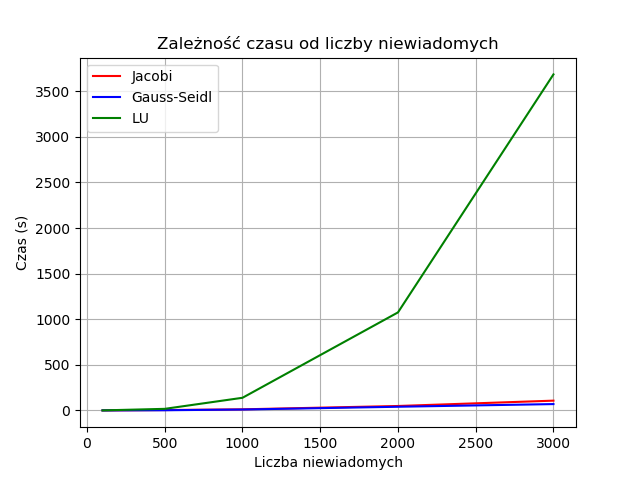
\includegraphics[scale=0.7]{wykres.png}
    \caption{ wykres zależności czasu od liczby niewiadomych dla metod Jacobiego, Gaussa-Seidla i LU}
\end{figure} \\
Dokładne czasy przedstawia poniższa tabela:
\begin{center} 
    \begin{tabular}  { | c | c | c | c |  }
        \hline
       Ilość iteracji & Jacobi & Gauss-Seidl & LU \\
       \hline
       100 & 0.09 & 0.06 & 0.11\\
       \hline
       500 & 3.88 & 1.81 & 17.10 \\
       \hline
       1000 & 11.69 & 9.63 & 138.44 \\
       \hline
       2000 & 48.42 & 40.09 & 1074.86 \\
       \hline
       3000 & 106.96 & 69.41 & 3685.58 \\
       \hline
    \end{tabular}
\end{center}
\section{Zadanie F}
Czas wykonywania obliczeń dla każdej z powyższych metod wzrasta wraz ze wzrostem liczby niewiadomych. Metoda bezpośrednia, faktoryzacja LU jest najdokładniejsza, ale zajmuje znaczną ilość czasu (przy 3000 niewiadomych czas wykonywania wynosi około godzinę). Metody iteracyjne nie są tak dokładne, ale wykonują się znacząco szybciej. Metoda Gaussa-Seidla wymaga mniejszej liczby iteracji i znajduje rozwiązanie szybciej niż metoda Jacobiego, dla każdego rozmiaru danych testowych. Warto zauważyć, że im większe dane, tym większa różnica pomiędzy metodami iteracyjnymi. \\
Z powyższych obserwacji można wywnioskować, że metody iteracyjne lepiej nadają się dla rozwiązywania układów równań z dużą liczbą niewiadomych. Jednak należy zauważyć, że może nastąpić sytuacja z zadania C, gdzie metody iteracyjne nie zbiegały się do rozwiązania. Wtedy jedyną opcją pozostaje rozwiązanie za pomocą metody bezpośredniej.
\end{document}